\section{RNN Computation Analysis} 
\label{sec:app}
In this section, we first discuss the limitation of BLAS-based LSTM on processor and spatial architectures.
Next, we discuss our implementation of loop-based LSTM on spatial architectures.
Table \ref{tab:legend_app} contains specifications for symbols and parameters
  used in this section.
\begin{table}[t]
  \vskip 0.15in
  \centering
  \scriptsize
  \begin{tabular}{p{0.6cm}m{3cm}m{3cm}}
  \toprule
    Symbol & Processor & Reconfigurable Hardware \\
    \midrule
    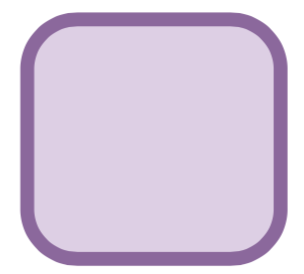
\includegraphics[width=0.03\columnwidth]{figs/innerloop.png} & Kernel & Inner Loop \\
    
\includegraphics[width=0.03\columnwidth]{figs/onchip.png} & Memory Hiearchy & On-chip Scratchpad \\
    
\includegraphics[width=0.03\columnwidth]{figs/reg.png} & Register File & Register \\
    
\includegraphics[width=0.1\columnwidth]{figs/unrollparm.png} & & Unrolling factor using multiple hardware compute blocks \\ \midrule
    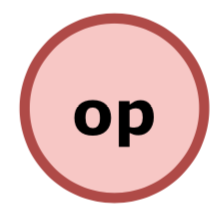
\includegraphics[width=0.03\columnwidth]{figs/vec.png} & \multicolumn{2}{L{6.5cm}}{Element-wise Operation} \\
    
\includegraphics[width=0.03\columnwidth]{figs/outerloop.png} & \multicolumn{2}{L{6.5cm}}{Outer Loop} \\
    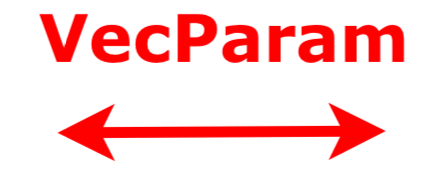
\includegraphics[width=0.1\columnwidth]{figs/vecparam.png} & \multicolumn{2}{L{6.5cm}}{Vectorization parameter for AVX or SIMD instructions} \\
    \midrule
    \midrule
    Parameter & \multicolumn{2}{l}{Specification} \\
    \midrule
    $hv$      & \multicolumn{2}{l}{Vectorization parameter on H} \\
    $hu$      & \multicolumn{2}{l}{Unrolling factor on H} \\
    $rv$      & \multicolumn{2}{l}{Vectorization parameter on R} \\
    $ru$      & \multicolumn{2}{l}{Unrolling factor on R} \\
    $G$       & \multicolumn{2}{l}{Number of gates in an RNN. For LSTM, G=4} \\
  \bottomrule
  \end{tabular}
  \caption{Specifications for symbols and parameters in Section \ref{sec:app}.}
  \label{tab:legend_app}
  \vskip -0.1in
  \end{table}

\begin{figure*}
  \centering
  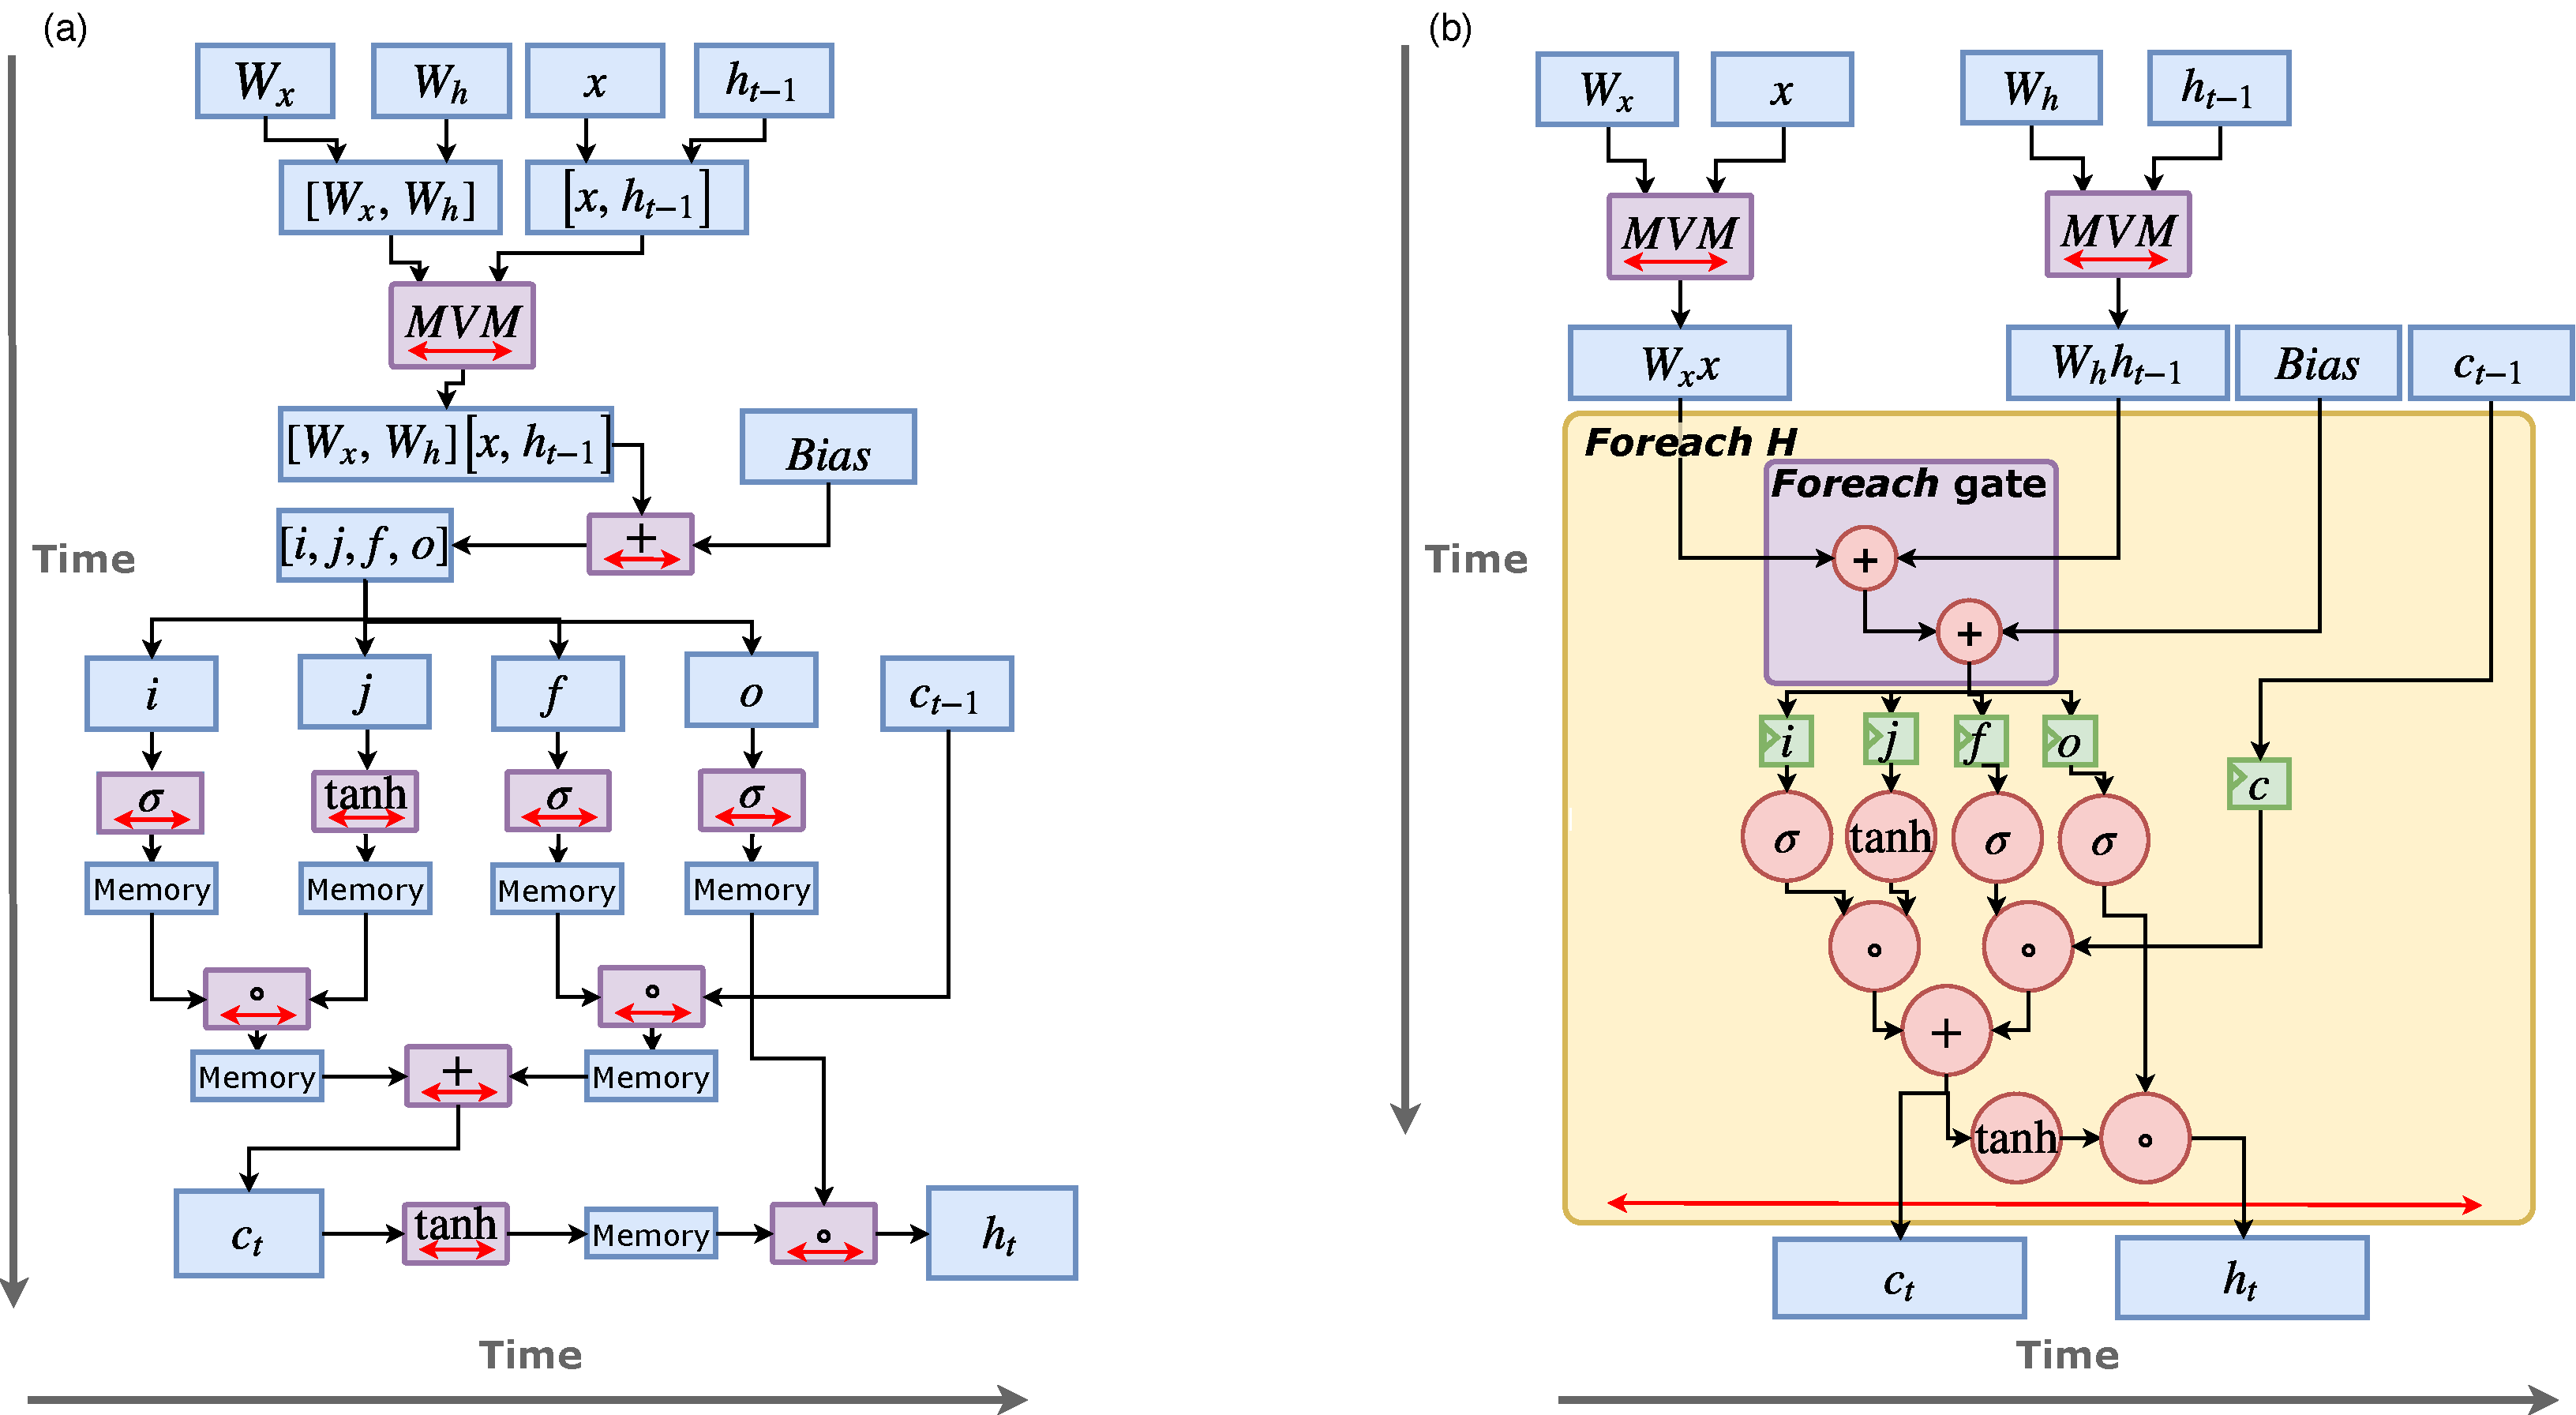
\includegraphics[width=1.5\columnwidth]{figs/cpugpulstm.pdf}
  \caption{Compute and memory layout of TensorFlow \texttt{BasicLSTM} cell on CPU (a) and \texttt{CudnnLSTM} cell on GPU (b).}\label{fig:tf_lstm}
\end{figure*}

\subsection{BLAS-based LSTM on Processor Architecture}
Modern Machine Learning frameworks, e.g.
  TensorFlow \cite{abadi2016tensorflow},
  divide the computation graph of an LSTM cell into BLAS kernels.
Then, the BLAS kernel is accelerated by calling low-level
optimized BLAS subroutines such as Intel BLAS Library on CPU
and NVBLAS Library on GPU.
Figure \ref{fig:tf_lstm} (a) shows the computation graph of a \texttt{BasicLSTM} cell in TensorFlow.
This implementation can lead to large memory footprint since all the intermediate results are
  materialized in memory.
A common strategy to tackle the issue is through fusing blocked kernels.
With TensorFlow's abstraction, this can only be achieved by
  expressing the entire RNN cell as an optimized kernel.
For example, TensorFlow provides \texttt{LSTMBlockFusedCell} and \texttt{GRUBlockCell} modules,
  which are the fastest TensorFlow implementations of RNN cells for CPU.
In practice, such implementation can provide significant performance improvement
  over the \texttt{BasicLSTM} implementation.
However, it is still very hard to saturate CPU compute capacity, potentially
due to the high synchronization overhead across threads.
Figure \ref{fig:tf_lstm} (b) shows the computation layout of TensorFlow with
cuDNN library \cite{chetlur2014cudnn} on GPU. cuDNN is an NVIDIA GPU
library for accelerating deep neural networks.
To minimize the data movement,
  cuDNN fuses all the vector-vector (VV) operations after MVM. Specifically, the bias add in
  Equation \ref{eq:1}, \ref{eq:2}, \ref{eq:3}, \ref{eq:4},
  and all the operations in Equation \ref{eq:5}, \ref{eq:6},
  are fused into one kernel.
Nevertheless, there are still intermediate buffers of size $H$
  between the MVM kernel and the element-wise operations.

Compared to the \texttt{BasicLSTM} implementation,
  \texttt{CudnnLSTM} eliminates most of large intermediate memories.
However, the MVMs of Equation \ref{eq:1}, \ref{eq:2}, \ref{eq:3}, \ref{eq:4} are all accelerated
with BLAS3 kernels, which performs only matrix-matrix level operations.
This turns MVM and VV bias add into Matrix Matrix Multiplication (MMM) and Matrix Matrix
Addition (MMA), which leads to serious underutilization of GPU.

Moreover, a processor-based architecture introduces large energy overhead of instruction
  decoding and scheduling.
GPU especially suffers from its power-hungry, high-throughput memory hierarchy.
For these reasons, both the CPU and GPU architectures are not suitable
  for energy-efficient, low-latency RNNs serving platforms.

\subsection{BLAS-based LSTM on Spatial Architecture}

Previous work has studied the capability of using an FPGA as a low-latency serving platform.
An FPGA has the flexibility of resizing MVM and VV units based on the application size.
In addition, MVM and VV units can be implemented with hardware pipelines,
  which removes the instruction scheduling and control overhead on a processor-based
  architecture.
The latest version of Intel Stratix 10 FPGA further boosts the compute power of FPGA
  with increasing number of hardened digital signal processing (DSP) blocks
  and on-chip memory capacity.
Microsoft Brainwave (BW) \cite{fowers2018configurable}
  is a state-of-the-art FPGA-based deep learning framework.

Figure \ref{fig:bw_lstm} shows BW's compute and memory layout.
In contrast to the CPU and GPU implementations, BW blocks the MVM along both
  row and column dimensions.
It then fuses the inner tiled MVM with element-wise non-linear functions.
Specifically for a matrix of size $H\times R$ and a vector of size $R$,
BW parallelizes the compute of multiple column tiles ($ru$, \# MV Tiles in the original paper) of size
$hv\times rv$ with multiple tiled engines, as shown in Figure \ref{fig:bwt} (a). 
Each tile engine contains $hv$ (native dimension) number of dot
product engines vectorized by $rv$ (lanes) and achieves one tile per cycle throughput. 
Parallel tiles along the row dimension are then fed into a pipelined reduction and accumulation
unit.
Immediately after the accumulation, the multi-function units (MFUs) execute the
element-wise operations on the $hv$ vector chunk produced by the accumulator.
Although BW's implementation still keeps the vectorized intermediate results, the size $hv$ is much
smaller than $H$ in \texttt{BasicLSTM} cell.
Nonetheless, with parallelization in $ru$,
  BW allocates lots of vectorized intermediate buffers that can still lead to energy inefficiency.
BW performs one MVM operation in $\ceil[\big]{\frac{H}{hv}}\ceil[\big]{\frac{R}{rv\cdot ru}}$
  iterations.

The MVM operations are executed on each gate of the LSTM sequentially.
Similarly, element-wise operations $hv$ using $\sigma, \tanh, \circ, +$ for the non-linear 
operators are also scheduled to execute on the vectorized multi-function units with size
of $hv$, as shown with the arrow in time in Figure \ref{fig:bw_lstm}.
To avoid DRAM communication overhead and improve compute density, Brainwave embeds MVM in a blocked floating-point format, 
where the vector of $hv$ values share a single 5-bit exponent and have distinct signs and 2-5 bit mantissa for
each value. As a result, they can achieve very dense low-precision compute and storage, with one
adder per $hv$ values and $hv$ multipliers for a vector of $hv$. The remaining operations are
performed in 16-bit precision.

When matrix dimensions cannot be divided by $hv$ and $rv\cdot ru$, Brainwave suffers from
underutilization of the compute FLOPS, as shown in Figure \ref{fig:bwt} (a).
The underutilization is worse with small problem sizes.
In addition, BW computes $W_xX$ and $W_hH$ separately rather than computing them with concatenated larger matrices,
  which can further aggravate the problem.
This might be because BW's abstraction does not allow partial updates of an vector
  but only $X$ is updated at the end of the step.


\subsection{Loop-based LSTM}
We have made the following observations
  from analyzing BLAS-based LSTM implementations:
\begin{enumerate}
\item 
  Constructing an LSTM cell's computation graph using BLAS subroutines
  introduces large intermediate buffers even when the kernels themselves are blocked.
  Each element on RNN cells' non-reduction dimension of the MVM ($H$)
  can be computed completely independently within one time step. This
  exposes the opportunity of fine-grain loop tiling and fusion across the
  entire LSTM kernel. 
\item MVM is the computation bottleneck in serving RNN cells. Spatial
  architecture allows us to distribute most of the compute resource to MVM 
  by parallelizing and pipelining MVM with element-wise operations.
\item Using low-precision operations can boost compute density and keep RNN
  weights on-chip to avoid high-latency DRAM communication. We need to introduce
  efficient low-precision support in the target spatial architecture without introduce
  too much overhead.
\end{enumerate}

To address the issue of large intermediate buffers, we fine-grain tile and fuse
MVM with non-linear functions. We refer to the computation for generating 
every single element in $c_t$ and $h_t$ as LSTM-1 operation, which can be computed
independently in a single step. LSTM-1 is composed of four independent dot products of 
the row vectors of the weight matrices with the input vector immediately followed by the 
element-wise operations on output of the dot product. The resulting $c$ and $t$ vectors are 
produced by computing LSTM-1 operations for $H+D$ iterations.

\label{sec:blaslstm}
 \begin{figure}
  \centering
  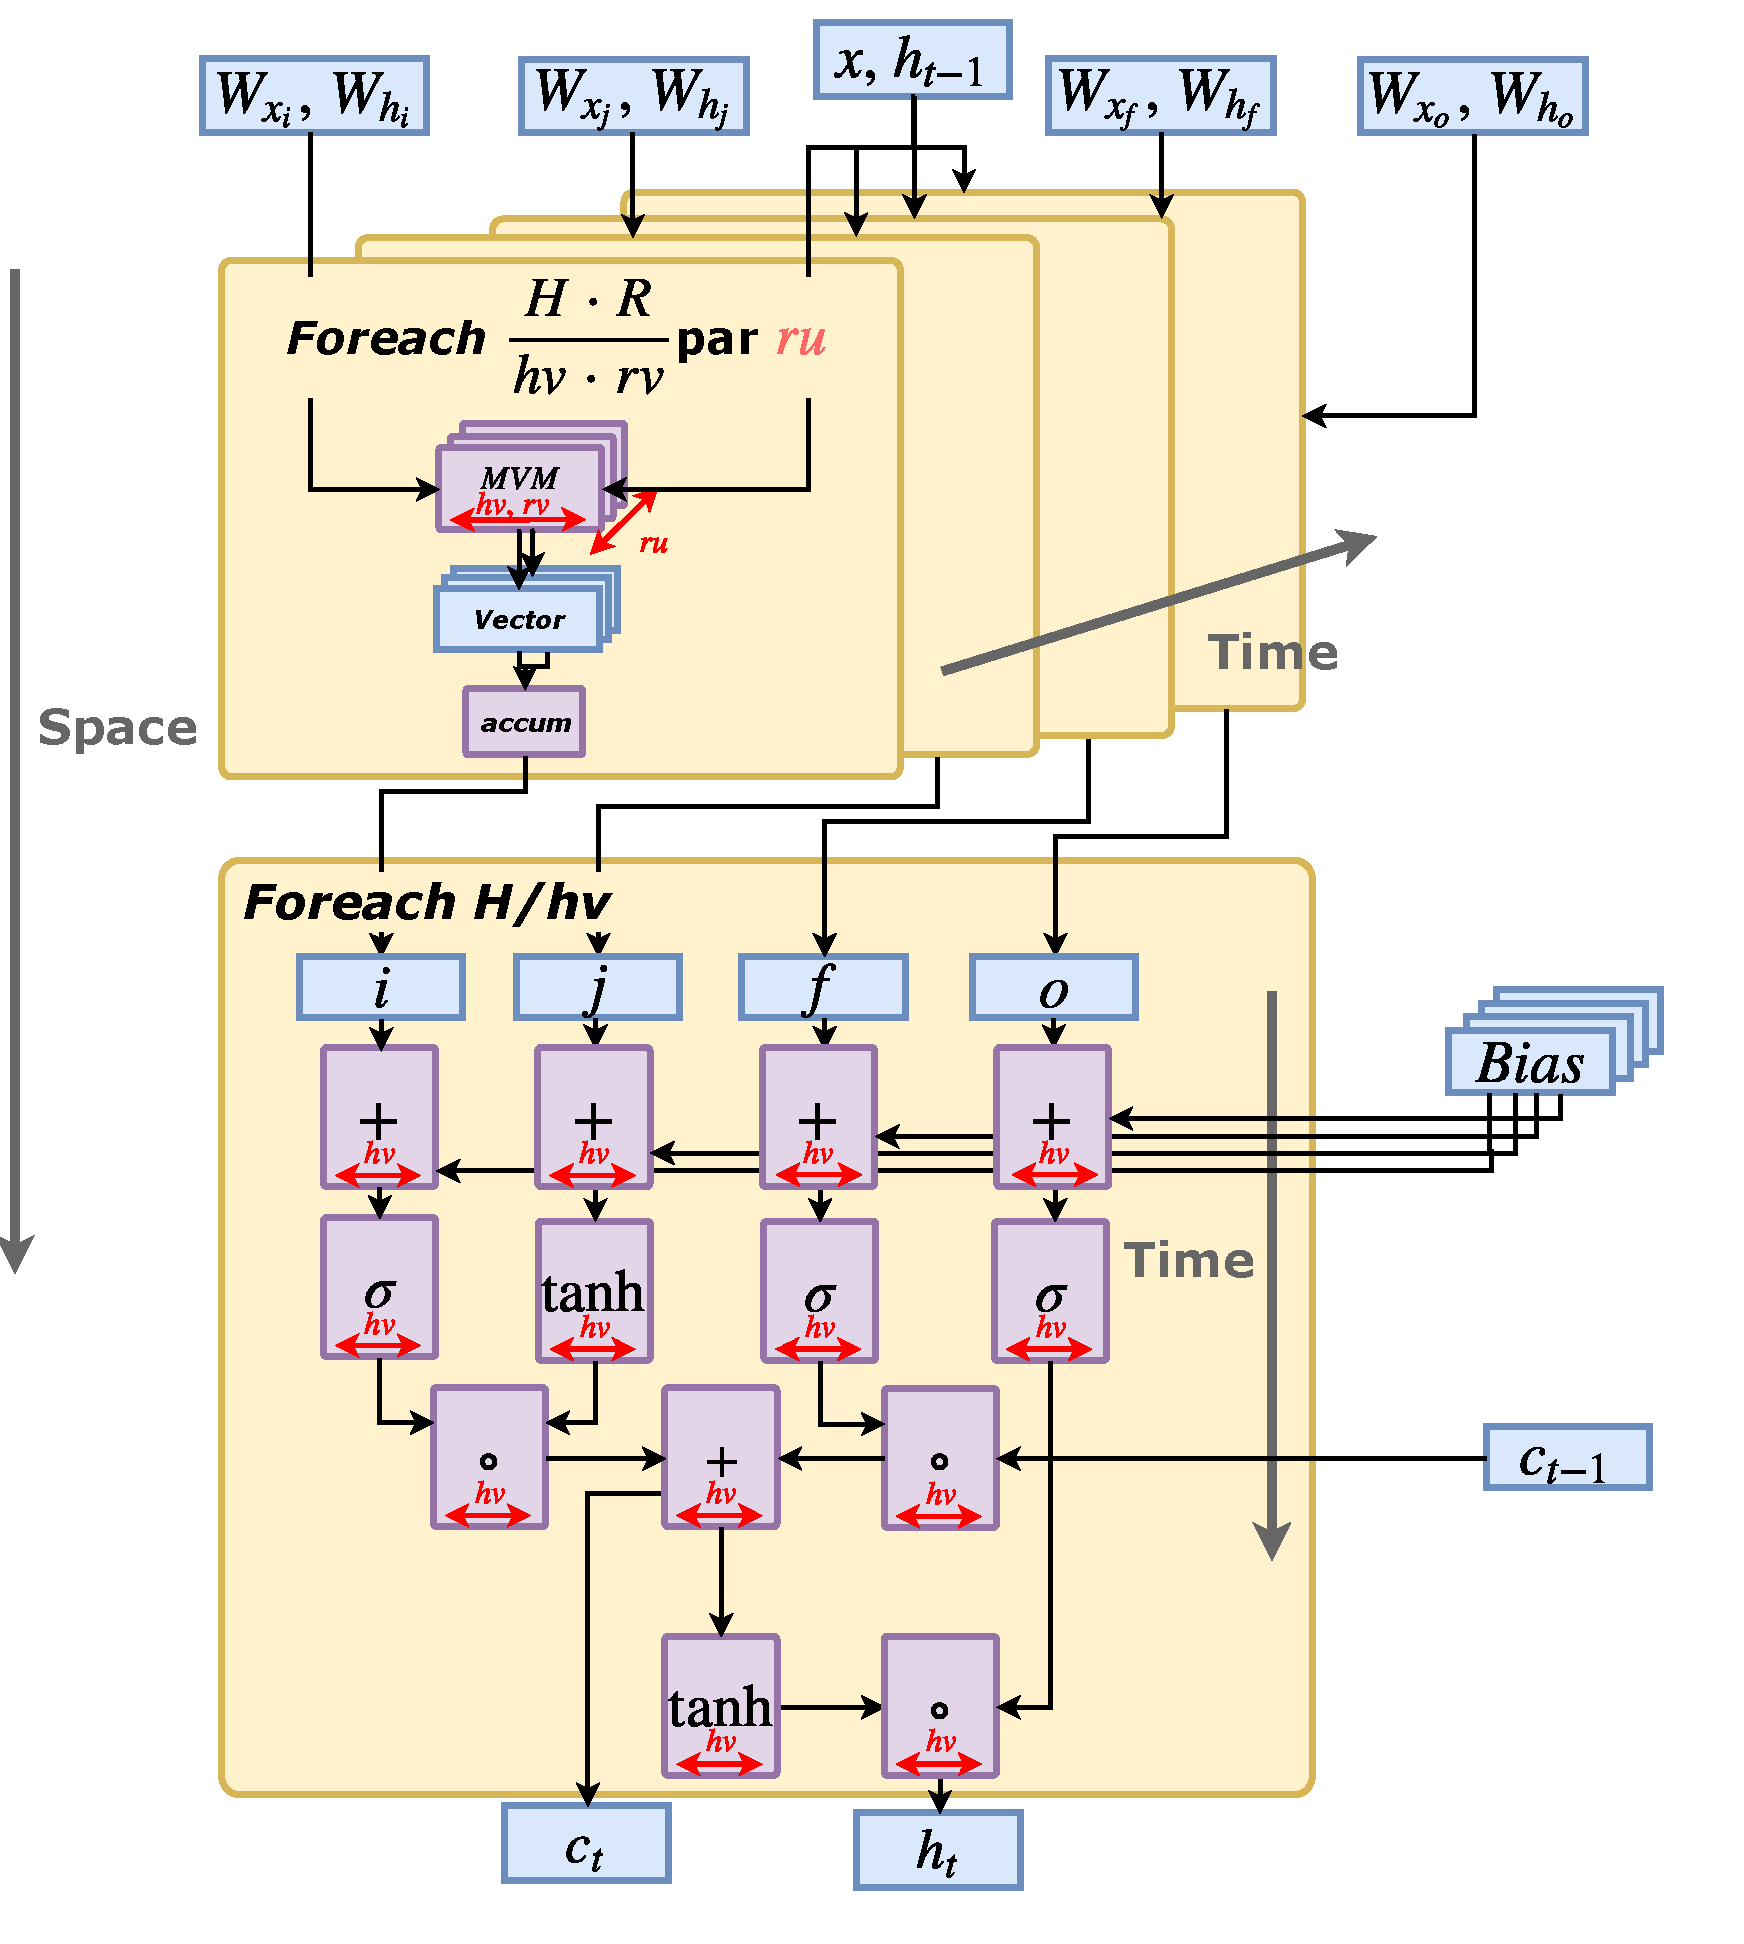
\includegraphics[width=0.8\columnwidth]{figs/bwlstm.pdf}
  \caption{Compute and memory layout of LSTM in Brainwave.}\label{fig:bw_lstm}
   \vspace*{-0.3in}
\end{figure}

\begin{figure}
 \centering
  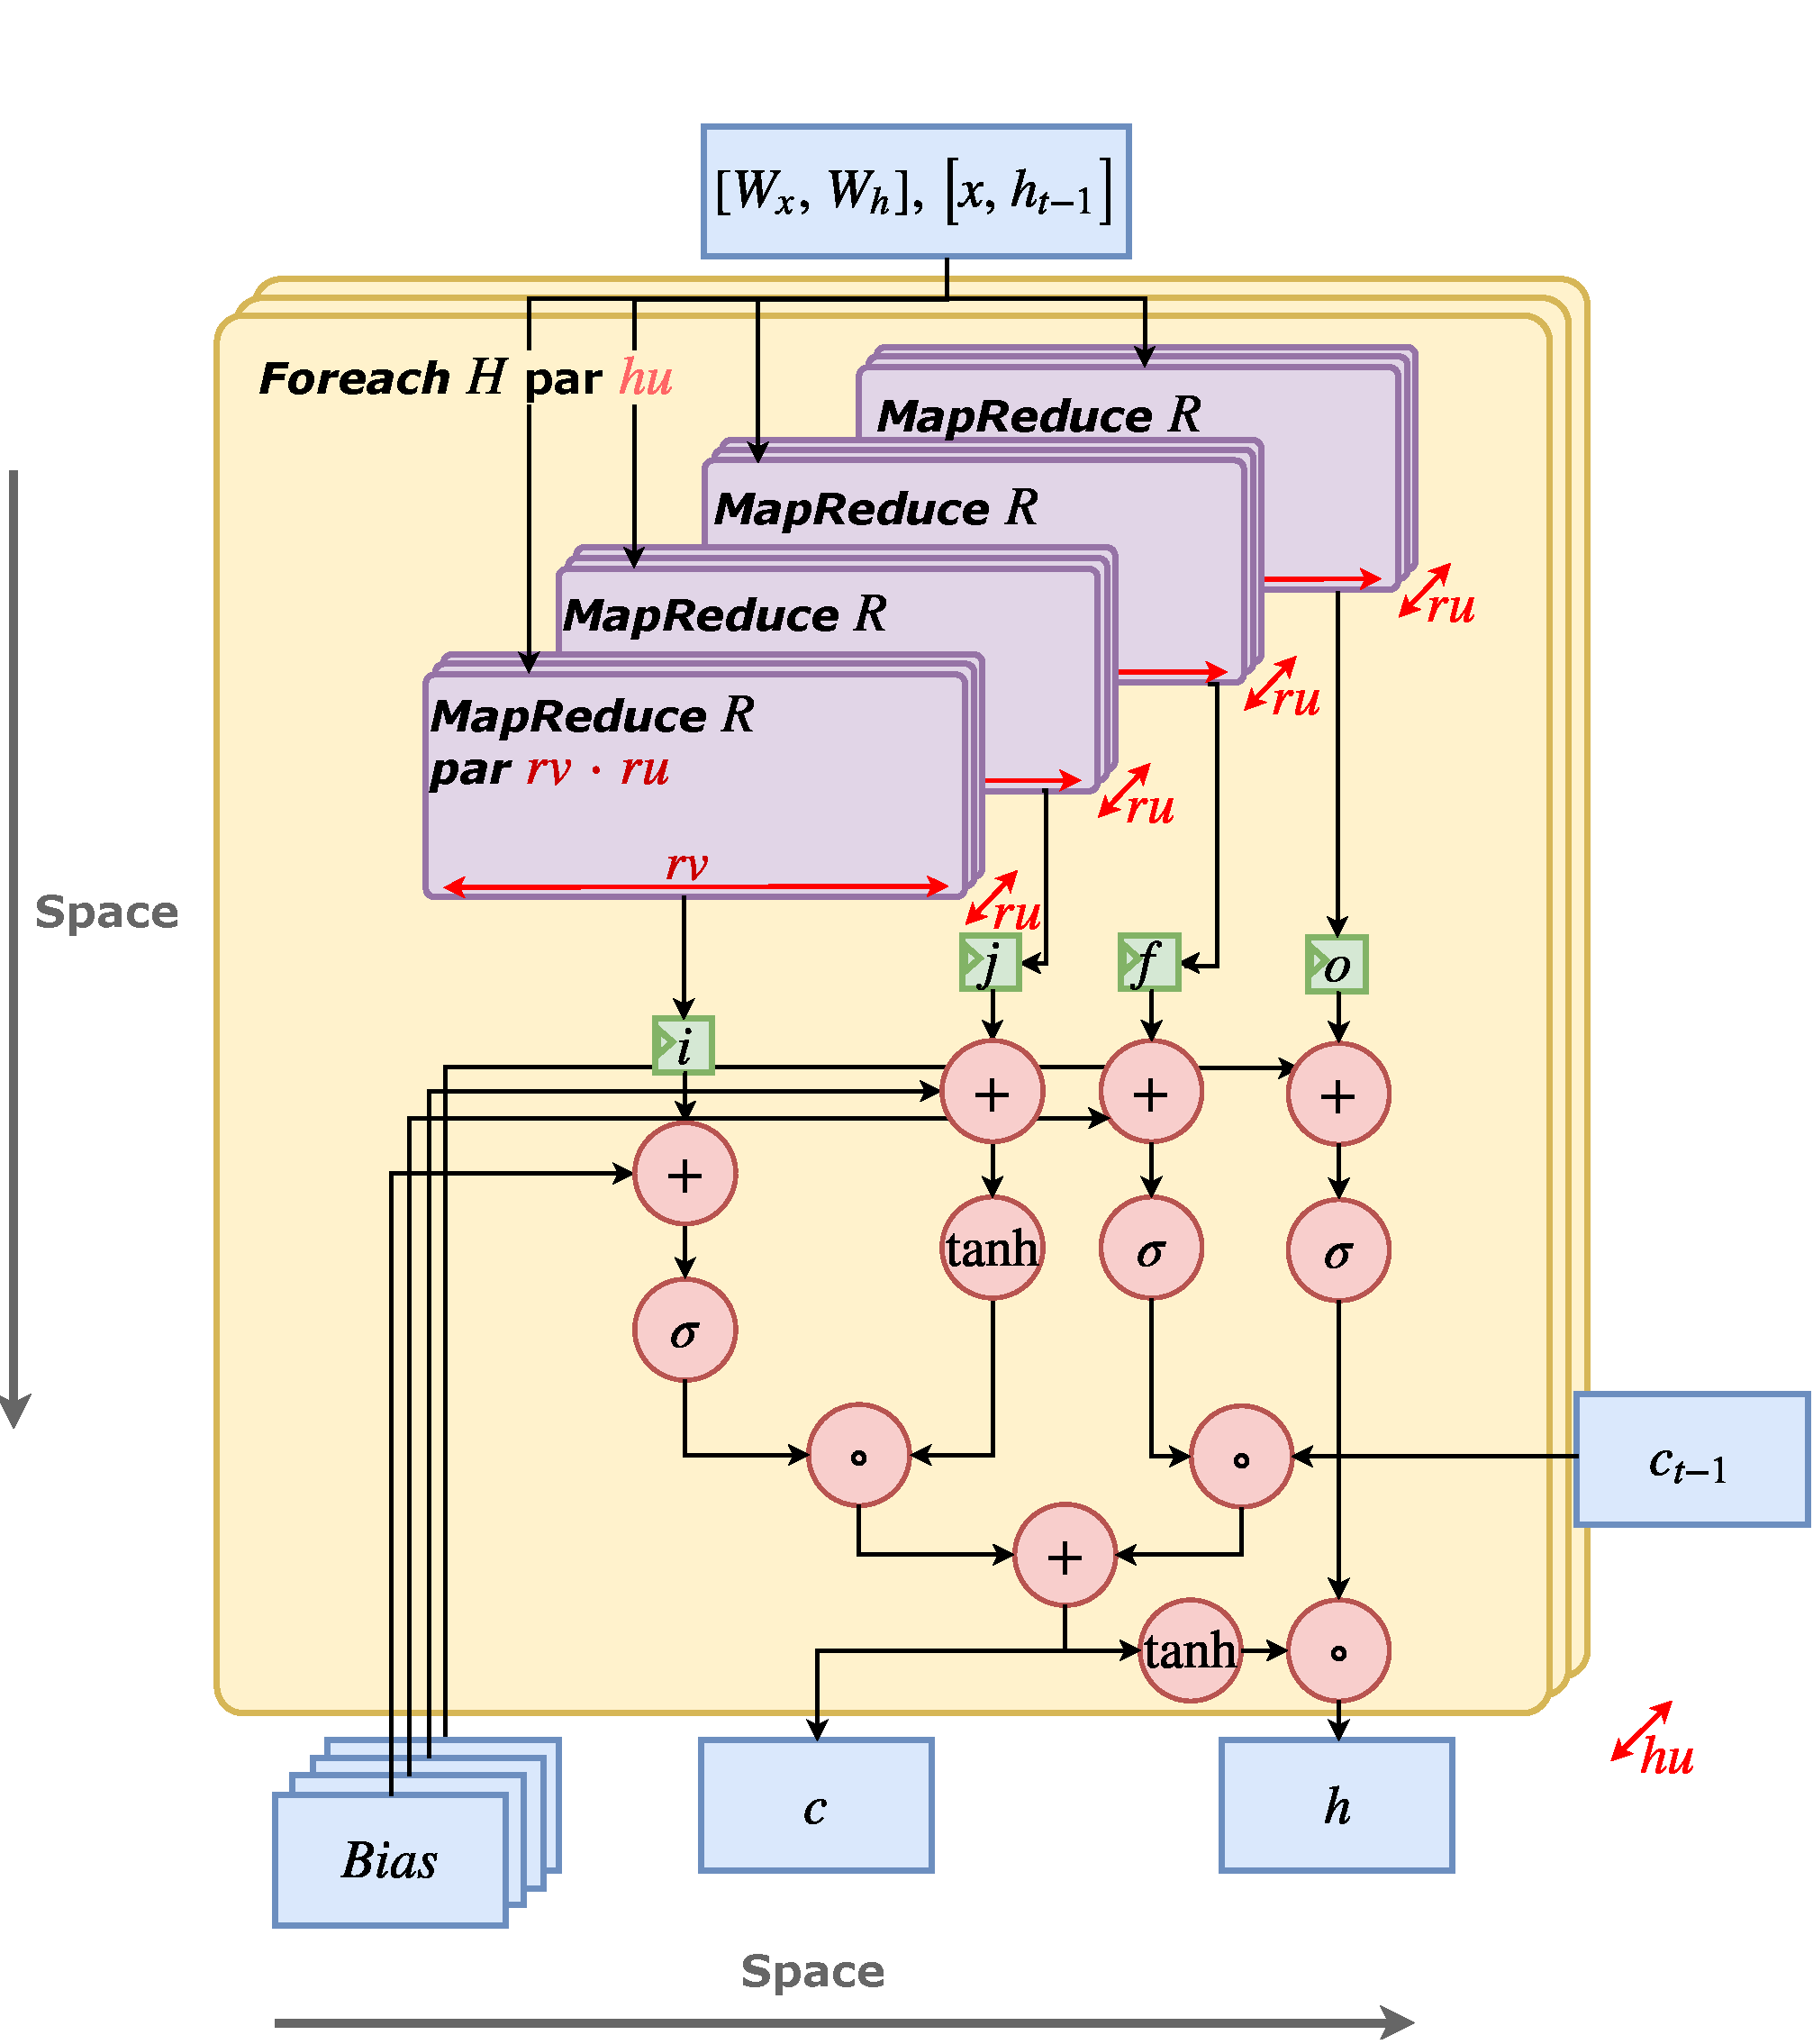
\includegraphics[width=0.9\columnwidth]{figs/splstm.pdf}
  \caption{Compute and memory layout of a loop-based LSTM design.}\label{fig:spatial_lstm}
  \vspace*{-0.2in}
\end{figure}
\begin{figure}
  \centering
  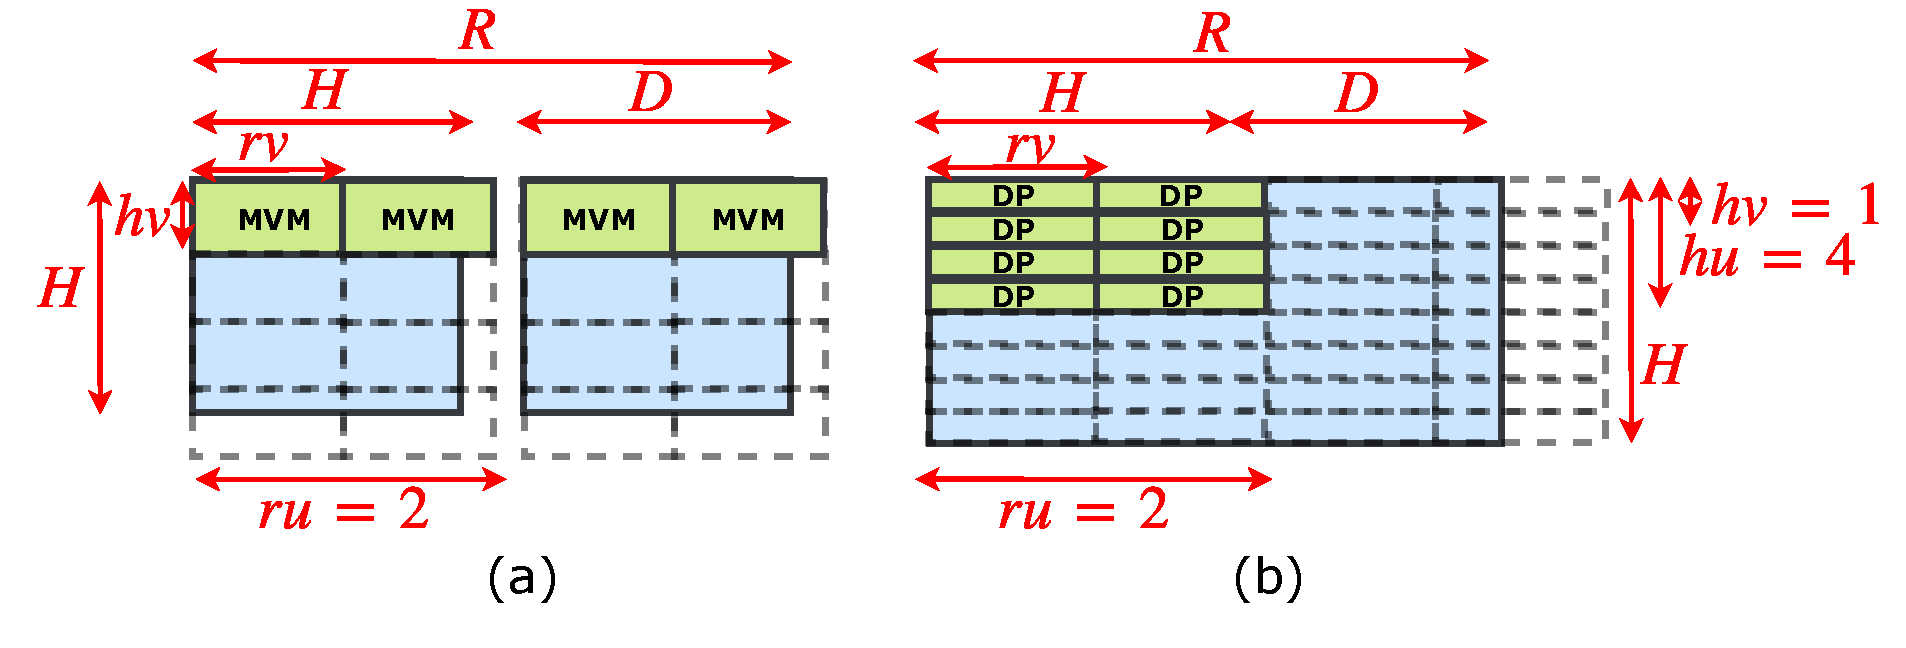
\includegraphics[width=\columnwidth]{figs/bwfrag.pdf}
   \caption{Fragmentation in an MVM-based design (a) and a loop-based design (b) in MVM.}\label{fig:bwt}
\end{figure}

As shown in Figure \ref{fig:spatial_lstm}, each MVM unit is replaced by a MapReduce unit to 
compute the tiled dot product.
Each MapReduce is vectorized by $rv$ with pipelined map function followed by a pipelined reduction tree.
$ru$ is the number of parallel MapReduce units. Results of $ru$ MapReduce blocks are reduced and 
accumulated with another reduction tree (not shown in Figure). Next, the dot product result is passed 
through a chain of function units for executing bias add and non-linear functions. Dot products, bias adds, 
and non-linear functions of the four gates can also be parallelized. Finally, the results of the four gates are pipelined
through a set of function units for element-wise operation in LSTM cell.
At the outer loop, LSTM-1 runs for $\frac{H}{hu}$ iterations,
  where $hu$ is the number of parallel LSTM-1 implementations.

In the loop-based design, all intermediate buffers are scalars as supposed to vectors. 
Regarding utilization, the loop-based LSTM design suffers from less underutilization due to unaligned problem size 
compared to the tiled MVM approach in BW. Figure \ref{fig:bwt} shows sources of such underutilizations.
An MVM approach design would suffer from 2-D fragmentation on both the $H$ and $D$ dimensions (Figure \ref{fig:bwt} (a)), whereas
the loop-based design only suffers from 1-D fragmentation on the $R$ dimension (Figure \ref{fig:bwt} (b)).

%Using BLAS terminology,
  %an LSTM-1 operation can be thought of as a new BLAS level-1 routine,
  %i.e. element-wise operations.
%In contrast, previous works mostly focus on optimizing level-2 or 3 routines.
%We find that optimizing at the lowest BLAS level allows us to utilize hardware resources more efficiently.
%In addition, using parallel patterns and loop constructs as the basic building block
  %offers sufficient abstraction and does not lead to much engineering overhead.
\begin{figure}
  \centering
  \newsavebox{\lstm}
  \begin{lrbox}{\lstm}
    \lstinputlisting[language=Spatial,linewidth=1.0\columnwidth]{code/lstm.scala}
  \end{lrbox}
  \begin{tabular} {c}
    \usebox{\lstm} \\
  \end{tabular}
  \caption{Example of LSTM in Spatial.}
\label{fig:spatial_app}
\end{figure}

Figure \ref{fig:spatial_app} shows a loop-based LSTM design implemented in Spatial.
\textbf{Foreach} is a loop construct with a lambda that takes loop iterator as input.
\textbf{Reduce} is a construct that executes MapReduce by taking a map function followed
by a reduction function. User declare explicit on-chip scratchpads and registers with
\textbf{SRAM} and \textbf{Reg}.
To enable fine-tuning an RNN application, we exposes loop vectorization factor $rv, hv$ and
unrolling factors $hu, ru$.
